\section{Rechengesetze}
\begin{multicols}{2}
\subsection{Potenzregeln}
\renewcommand{\arraystretch}{2}
\begin{tabular}{|c|c|}
	\hline $a^0=1$ & $a^-n= \frac{1}{a^n}$\\
	\hline $a^m \cdot a^n = a^m+n$ & $\frac{a^n}{a^m}= a^n-m$\\
	\hline $(a^n)^m = a^n*m$ & $(\frac{a}{b})^n = \frac{a^n}{b^n}$\\
	 \hline $a^n*b^n = (ab)^n$ & $a^\frac{b}{n}= \sqrt[n]{a^b}$\\
	 \hline
\end{tabular}

\subsection{Wurzelregeln}
\renewcommand{\arraystretch}{2}
\begin{tabular}{|c|c|}
	\hline $\sqrt[n]{a^n}= (\sqrt[n]{a})^n$ & $\sqrt[n]{\frac{a}{b}} = \frac{\sqrt[n]{a}}{\sqrt[n]{b}}$\\
	\hline $\sqrt[n]{a^x}=(\sqrt[n]{a})^x$ & $a\sqrt[n]{x} + b \sqrt[n]{x} = (a+b)\sqrt[n]{x}$\\
	\hline $\sqrt[n]{a \cdot b} = \sqrt[n]{a} \cdot \sqrt[n]{b}$ & $a\sqrt[n]{x} - b \sqrt[n]{x} = (a-b)\sqrt[n]{x}$\\
	\hline $\sqrt[n]{\sqrt[m]{a}}= \sqrt[n \cdot m]{a}$ & $\sqrt[n]{a^x}= a^\frac{x}{n}$ \\
	\hline
\end{tabular}
\end{multicols}

\subsection{Logarithmusregeln}
\begin{minipage}{10cm}
	\begin{tabbing}
		xxxxxxxxxxxxxxxx \= xxxxxxxxxxxxxxxx \= \kill
		$lg(x) = \log_{10} x$ \> $ln(x) = \log_{e} x$ \> $lb(x) = \log_{2} x$
	\end{tabbing}
	\renewcommand{\arraystretch}{2}
	\begin{tabular}{|c|c|}
		\hline $\log{xy} = \log{x} + log{y}$ & $\log{\sqrt[n]{x}}=\log{x^\frac{1}{n}}$\\
		\hline $\log{\frac{x}{y}}= \log{x} + log{y}$ & $\log{x^y}= y\log{x}$ \\
		\hline $\log{\sqrt[n]{x}}= \frac{\log{x}}{n}$ & $\log{1}=0$\\
		\hline
	\end{tabular}
\end{minipage}
\begin{minipage}{5cm}
	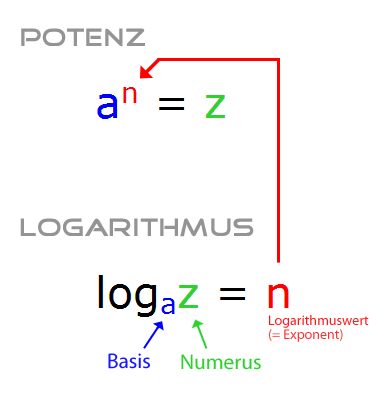
\includegraphics[width=4cm]{images/potenz_logarithmus.png}	
\end{minipage}

\begin{multicols}{2}
	\subsection{Binom}
	\renewcommand{\arraystretch}{2}
	\begin{tabular}{|c|}
		\hline $a^2+2ab+b^2 = (a+b)(a+b)$\\
		\hline $a^2-2ab+b^2 = (a-b)(a-b)$\\
		\hline $a^2-b^2= (a+b)(a-b)$\\
		\hline $(a \pm b)^3 =a^3 \pm  3 a^{2} b + 3 a b^2 \pm b^3 $\\
		\hline $(a \pm b)^4 =a^4 \pm  4 a^{3} b + 6a^2b^2 \pm 4 a b^3 +	b^4$\\
		\hline
	\end{tabular}
	
	\subsection{Quadratische Gleichung}
	\begin{tabbing}
		xxxxxxxxxxxxxxxxxxxx \= \kill
		$ax^2+bx+c=0$ \> $x_{1,2} = \dfrac{-b \pm \sqrt{b^2 - 4ac}}{2a}$
	\end{tabbing}
\end{multicols}
\clearpage
\pagebreak
\subsection{Partialbruchzerlegung}
\[f(x)=\frac{x^2+20x+149}{x^3+4x^2-11x-30} \Rightarrow \; \begin{array}{l}\text{Nenner faktorisieren}
\end{array} \Rightarrow
x^{3}+4x^{2}-11x-30=(x+2)(x^{2}+2x-15)=(x+2)(x+5)(x-3)\] Ansatz:
\[f(x)=\frac{x^2+20x+149}{x^3+4x^2-11x-30}=\frac{A}{x-3} + \frac{B}{x+2} + \frac{C}{x+5}=
\frac{A(x+2)(x+5)+B(x-3)(x+5)+C(x-3)(x+2)}{(x-3)(x+2)(x+5)}\]
Gleichungssystem aufstellen mit beliebigen $x_i$-Werten (am Besten Polstellen oder 0,1,-1 wählen):
\[\begin{array}{l}x_1=3:\;-9+60+149=A\cdot5\cdot8\;\;\;\Rightarrow A=5\\
x_2=-2:\;-4-40+149=B(-5)\cdot3\; \Rightarrow B=-7\\
x_3=-5:\;-25-100+149=C(-8)(-3) \Rightarrow C=1 \end{array} \Rightarrow
f(x)=\frac{5}{x-3}-\frac{7}{x+2}+\frac{1}{x+5}\] weitere Ansätze für andere
Typen von Termen: \[f(x)=\frac{5x^2-37x+54}{x^3-6x^2+9x}=\frac{A}{x}+\frac{B}{x-3}+\frac{C}{(x-3)^2}=\frac{A(x-3)^2+Bx(x-3)+Cx}{x(x-3)^2}\]
\[f(x)=\frac{1,5x}{x^3-6x^2+12x-8}=\frac{A}{x-2}+\frac{B}{(x-2)^2}+\frac{C}{(x-2)^3}=\frac{A(x-2)^2+B(x-2)+C}{(x-2)^3}\]
\[f(x)=\frac{x^2-1}{x^3+2x^2-2x-12}=\frac{A}{x-2}+\frac{Bx+C}{x^2+4x+6}=\frac{A(x^2+4x+6)+(Bx+C)(x-2)}{(x-2)(x^2+4x+6)}\]


Variante mit Koeffizientenvergleich: \\
\begin{minipage}{9cm}
	\[F(s) = \frac{1}{s(s^2+6s+13)} = \frac{A}{s} + \frac{Bs+C}{s^2+6s+13}\]
	\[1 = A(s^2+6s+13) + s(Bs+C)\] 
	\[1 = s^2(A+B) + s(C+6A) + 13A\] 
	\[\Rightarrow 1 = 13A; (A+B)=0; (C+6A)=0\]
	\[\Rightarrow A=\frac{1}{13}; B=-\frac{1}{13}; C=-\frac{6}{13}\]
\end{minipage}
\begin{minipage}{9cm}
	$s^2: A+B = 0$\\
	$s^1: 6A+C =0$\\
	$s^0: 13A = 1$
\end{minipage}

\subsection{Hornerschema}
\begin{minipage}[t]{9cm}
	- Pfeile $\Rightarrow$ Multiplikation\\
	- Zahlen pro Spalte werden addiert\\
	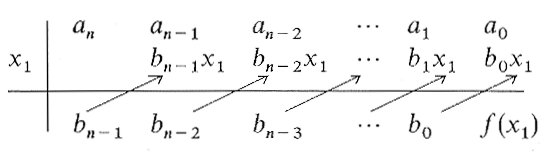
\includegraphics[width=6cm]{images/hornerschema_1.png}\\
	$x_1 \Rightarrow$ Nullstelle (muss erraten werden!!)\\
	oberste Zeile = zu zerlegendes Polynom			
\end{minipage}
\begin{minipage}[t]{9cm}
	\textbf{Beispiel:}\\
	$f(x) = x^3-67x-126$\\
	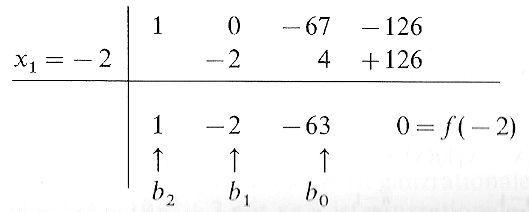
\includegraphics[width=6cm]{images/hornerschema_2.png}\\
	$\Rightarrow f(x) = (x-x_1)(b_2x^2 + b_1x + b_0) = (x+2)(x^2-2x-63)$	
\end{minipage}
\subsection{Winkelmasse}
\begin{tabular}{|l|l|l|}
	\hline & \textbf{Gradmass} & \textbf{Bogenmass}\\
	\hline \textbf{Einheit}& Grad, ° & Radiant, rad\\
	\hline \textbf{Vollwinkel}&  360° & 2$\pi$ rad\\
	\hline \textbf{Umrechnung} & $°= \frac{360}{2\pi} \cdot rad$ & $rad= \frac{2\pi}{360} \cdot °$\\
	\hline
\end{tabular}
\clearpage
\pagebreak